\chapter{\label{ch6-reduction}Waveform Processing} 

\minitoc

\section{Introduction}

Methods for retrieving information about the Cherenkov shower have been a primary component of the Imaging Atmospheric Cherenkov Technique since its inception. Early techniques such as those used in the first observation of TeV Gamma rays from the Crab nebula \cite{Weekes1989} are still utilised in modern \glspl{iact}. These techniques are also applicable to \gls{cta} telescopes, and as \gls{cta} is a large consortium which consists of the worldwide \gls{iact} community, the developers of advanced waveform reduction and shower reconstruction approaches used by previous \glspl{iact} have prepared them for use within \gls{cta} (for example, the ImPACT shower reconstruction technique developed by \cite{Parsons2014}. However, as:
\begin{enumerate}[label=(\alph*)]
	\item \gls{cta} will consist of the most advanced \glspl{iact} to date, with higher shower imaging resolution and telescope multiplicity than has previously been available,
	\item the capabilities of digital signal processing have significantly increased in the past decade,
\end{enumerate}
the opportunity for more advanced and more successful algorithms exists for \gls{cta}. Some efforts have already been made to develop novel approaches, such as one that utilises decision trees for the \textgamma-hadron discrimination \cite{Ohm2009}, or one that utilises convolutional neural networks to reconstruct the shower's direction \cite{Shilon2018}. However, it is an aspect that is expected to constantly evolve and improve during the lifetime of \gls{cta}. In this chapter I will provide insight into the existing and in-development reduction techniques utilised to extract the Cherenkov shower signal from the waveforms, and my involvement in designing a charge-extraction technique for \gls{chec-s}. I will also provide a brief overview of the shower reconstruction methods typically used with \glspl{iact}. With regards to the \gls{cta} data levels (Figure~\ref{fig:dataflow}), this chapter is mostly concerned with the steps from \textit{DL0} to \textit{DL2}.

\section{Charge Extraction Methods}

\begin{figure}
	\centering
    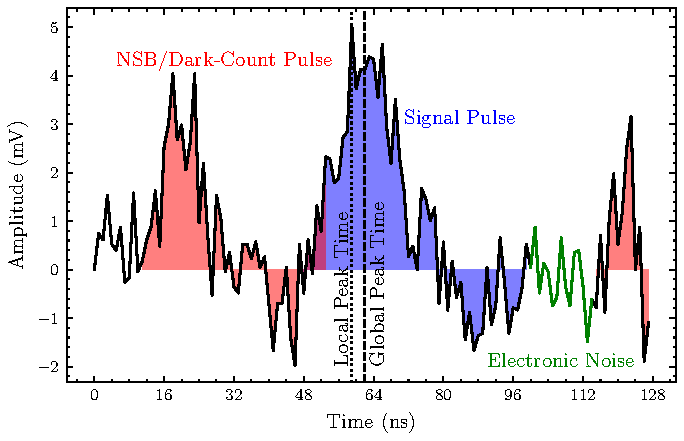
\includegraphics[width=\textwidth]{annotated_wf_3pe} 
	\caption[Annotated waveform.]{A waveform from CHEC-S lab data, illuminated by the laser with the filter wheel set to give an average expected charge of \SI{3}{\pe}. The waveform is annotated with the different components that contribute to the charge extraction. Although the electronic noise is only highlighted at one section, it affects every sample. Further information about the different contributors to the waveform can be found in Section~\ref{section:readout_characteristics}}
	\label{fig:annotated_wf_3pe}
\end{figure}

The immediate step after the waveform calibration is the extraction of signal (also sometimes referred to as charge) from the waveforms provided by the individual cameras. As a result of the low-level calibration detailed in Chapter~\ref{ch5-calibration}, the waveforms from each \gls{cta} camera exist in a common state, with no remaining dependencies on the electronics they were produced by. Therefore, the extraction techniques are typically applicable to all \gls{cta} cameras. 

The extraction of signal from a waveform is a very generic problem, allowing for the utilisation of common signal processing techniques that are not unique to Cherenkov shower analysis. The goal is to extract the majority of signal from the pulse created by the Cherenkov shower light, while simultaneously limiting the inclusion of noise factors\otherch{reference where noise talked about, talk about all the contributing factors (noise etc.) to waveforms in ch2}. Figure~\ref{fig:annotated_wf_3pe} shows a \gls{chec-s} waveform which contains both signal and noise. Two quantities are extracted in this stage: the signal charge in each pixel, and the signal arrival time per pixel. 

The total signal charge in a pixel,\final{Check all i.e. and e.g. for spaces} i.e.\@ the total number of photo-electrons released from the \gls{pmt}'s photocathode, is proportional to the total area below the pulse corresponding to the Cherenkov photons (blue area of Figure~\ref{fig:annotated_wf_3pe}). If the waveforms were completely free of noise, and the readout window was large enough to capture the full Cherenkov signal, a simple integration of the entire readout would be a satisfactory approach for obtaining the signal charge. However, as we do not have the luxury of perfect waveforms, more complex methods are required. Charge extraction algorithms typically consist of two aspects: how the signal pulse is found, and how the pulse is integrated.

\subsection{Peak Finding} \label{peakfinding}

Two factors must be considered when finding the signal pulse of a Cherenkov shower. Firstly, the majority of camera pixels will not contain any Cherenkov signal while still containing noise. A peak finding technique that assumes a signal exists in the readout will be biased, as it will mistake the noise for a signal. Secondly, due to the nature of Cherenkov showers (Chapter~ \otherch{reference where the time gradient of Cherenkov showers are described}), the Cherenkov signal will have different arrival times between pixels due to the time evolution of the Cherenkov image. This time gradient across the image is especially apparent for high-energy showers at a large core distance from the telescope. The most successful peak-finding technique is one that best accounts for those two factors. Some simple techniques used to define a peak time from a waveform include:
\begin{itemize}
	\item \textbf{Local Peak Finding}: Each waveform is treated independently from the others. The maximum point in the waveform is treated as the peak/arrival time. This approach is intrinsically biased to assume every waveform contains a signal; therefore, in the absence of a Cherenkov signal, the largest noise pulse will be extracted, resulting in a higher total charge than should be obtained.
	\item \textbf{Global Peak Finding}: The waveforms from each pixel are combined into an average waveform, from which the maximum sample is treated as the peak time for every pixel. This technique is only useful if a large portion of the camera is simultaneously illuminated, such as by a laser in the case of lab commissioning and calibration runs.
	\item \textbf{Neighbour Peak Finding}: The waveforms from neighbouring pixels to the pixel-of-interest are combined into an average waveform. The maximum sample in the average waveform is treated as the peak time for the pixel-of-interest. This technique is often preferred for Cherenkov images as it has a reduced charge bias (especially if the pixel-of-interest's waveform is not included in the average); pixels with Cherenkov signal typically have neighbours that also contain Cherenkov signal at a correlated time, while the neighbours of empty pixels only contain random noise, and therefore a peak time that is uncorrelated to the noise is chosen.
	\item \textbf{Fixed Peak Value}: Due to a reliable definition of the camera trigger and subsequent electronic chain, the position of the pulse in the waveform could consistently be known a priori, allowing for a fixed peak time. However, this method requires a larger integration window size in order to capture the full pulse in the tail of the Cherenkov shower, which occur at a later time than the initial photons which trigger the camera. As a result, a larger amount of noise will be included in the integration window. However, this technique usually contains the least bias, as no signal is assumed to exist.
\end{itemize}

 A more complex peak-finding technique is the \textit{Gradient Peak Finding} approach. This approach was designed for the VERITAS telescope \cite{Holder2005}\cite{Cogan2006}\cite{Cogan2007}, but is applicable to any \gls{iact} telescope that allows the dynamic specification of an integration window. \textit{Gradient Peak Finding} utilises the gradient profile of the photon arrival time for gamma-induced Cherenkov showers, described in Section~\ref{section:photon_arrival_time} and illustrated in Figure~\change{chec-m pulse time figure}. This peak-finding technique is a two-pass approach performed by first extracting the signal using one of the other methods. The pulse-timing information contained within the pixels that survive the image cleaning (Section~\ref{section:image_parametrisation}) can then be used to obtain a relation between ``distance along primary image axis'', $D_{ax}$, and the pulse time, $T_0$. Figure~\change{figure with geometry} illustrates the geometry of $D_{ax}$ with respect to the pixel position. Using the obtained relation between $D_{ax}$ and $T_0$, an example of which is shown in Figure~\change{figure of Dax versus T0 for checm figure}, an unbiased pulse time is obtained for each pixel depending on its position along the image axis.

These peak-finding methods have been described in relation to the maximum of the signal pulse, however they may instead use other characteristic positions of the pulse, such as the half-maximum time on the rising edge, or the centre of gravity of the pulse. Additionally, more advanced peak-finding techniques may up-sample (possibly by zero-padding in the frequency domain via a Fourier transform) or interpolate the signal to obtain a more precise peak time \cite{Cogan2006, Cogan2007}, or even apply low-pass filters in order to remove low frequency baseline noise. The peak finding should be done in conjunction with any timing corrections (Section~\ref{section:timing_corrections}) that may be required.

\subsection{Integration}

Once the peak time has been obtained, the simplest approach to extract the signal is to define an integration window centred about this time. The size of the window needs to be large enough to capture sufficient signal from the pulse, but small enough that not too much noise (\gls{nsb}, dark counts, afterpulsing) is included within the window, thereby maximising the signal-to-noise. Additionally, the camera's pulse shape may not be symmetric, so a better signal-to-noise may be achieved by shifting the window a few samples with respect to the peak time. The optimal integration window size and shift for the \gls{chec-s} waveforms is found to be 5 samples and 2 samples (i.e.\@ \SI{5}{ns} and \SI{2}{ns}\otherch{mention 1 sample == 1 ns in ch2}), respectively, according to the investigations performed in \ref{a3-extractors}.

Beyond the simple ``boxcar'' integrator method (where every sample integrated has a weight of 1), other more advanced strategies may be used to extract the charge. One example is the fitting of the waveform in order to extract the signal pulse, either with an analytical description of the expected pulse or with a more unconstrained description, such as a cubic spline. A second advanced approach is the use of digital filters, which can be used in combination with knowledge of the pulse shape to robustly extract the signal even in the presence of high frequency noise with a large amplitude. Such a technique has been designed and adopted for \gls{gct}, referred to as the \textit{Cross-Correlation} method. 

\subsubsection{Cross Correlation} \label{section:crosscorrelation}

\begin{figure}
  \begin{subfigure}[b]{0.32\textwidth}
    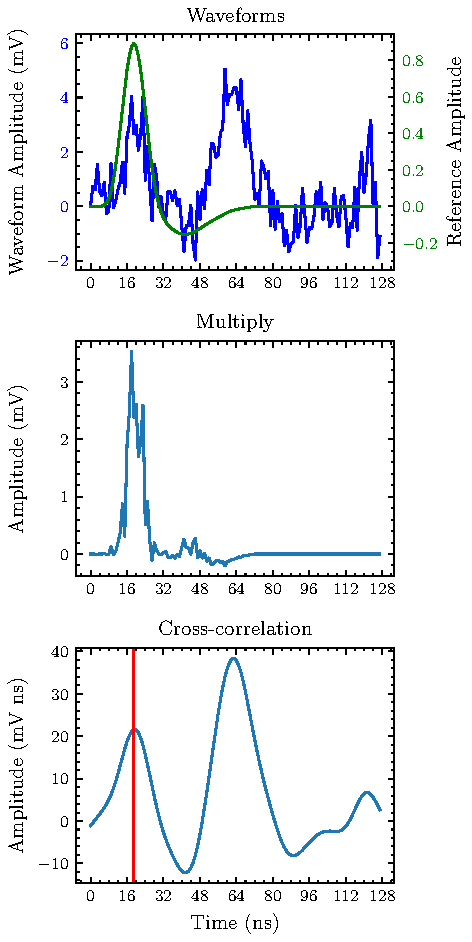
\includegraphics[width=\textwidth]{cc_tnsb}
    \caption{}
    \label{fig:cc_tnsb}
  \end{subfigure}
  \hfill
  \begin{subfigure}[b]{0.32\textwidth}
    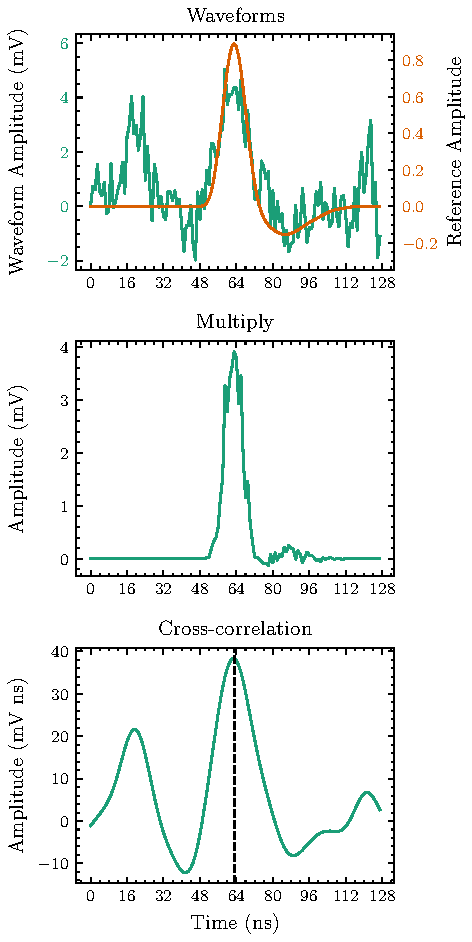
\includegraphics[width=\textwidth]{cc_tmax}
    \caption{}
    \label{fig:cc_tmax}
  \end{subfigure}
  \centering
  \begin{subfigure}[b]{0.32\textwidth}
    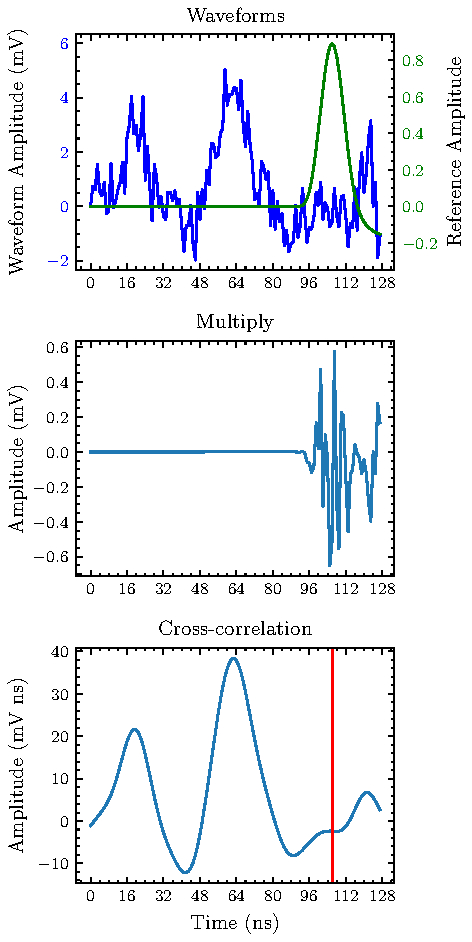
\includegraphics[width=\textwidth]{cc_tnoise}
    \caption{}
    \label{fig:cc_tnoise}
  \end{subfigure}
  \caption[Cross correlation stages.]{The three stages involved in obtaining the cross Correlation of a waveform with the reference pulse. The waveform investigated is the same one shown in Figure~\ref{fig:annotated_wf_3pe}. The stages are shown for three time displacements (Equation~\ref{eq:cc1}): on an NSB/dark-count pulse before the signal (a), at the time of the signal (b), and at a time where there is only the baseline (c). The top panels show the waveform and the reference pulse shifted by the time displacement. The middle panels show the multiplication of the two traces in the first panel. The bottom panel shows the cross correlation for all time displacements. The value of the cross correlation at the time displacement shown by the red line is obtained by summing all the samples from the trace in the middle panel.}
    \label{fig:cc}
\end{figure}

Cross-correlation is a common signal processing technique used as a measure of the similarity between two signals as a function of the displacement in time applied to one of the signals. Given a continuous function $f(t)$ defined between $0 \le t \le T$ and a second continuous function $g(t)$, the cross-correlation between the two functions ($f \star g$) is defined as 
\begin{equation} \label{eq:cc1}
(f \star g)(\tau) = \int_0^T \overline{f}(t)g(t + \tau)dt,
\end{equation}
where $\overline{f}(t)$ is the complex conjugate of $f(t)$ and $\tau$ is the time displacement (also referred to as the ``lag'') between the two functions \cite{wolfram-crosscorrelate}. In descriptive terms, as $\tau$ increases, $g(t + \tau)$ will slide past $f(t)$. The cross-correlation for a value of $\tau_1$ is then the integral across $t$ of the product between $f(t)$ and $g(t + \tau_1)$. For a discrete function that is real-valued, such as a sampled waveform, Equation~\ref{eq:cc1} can instead be defined as
\begin{equation} \label{eq:cc2}
(f \star g)\lbrack n \rbrack = \sum_{m=0}^N f\lbrack m \rbrack g\lbrack m + n\rbrack,
\end{equation}
where $N$ is the total number of samples in the waveform and $n$ is the sample displacement from sample $m$. 

Through utilising a template of the expected pulse shape in the absence of noise (hereafter referred to as the ``reference pulse''), features inside the waveform that are correlated with the reference pulse shape are emphasized, while features that are not, such as the electronic noise, are suppressed. Therefore, the peaks in the cross correlation correspond to the displacements where the signals match best, and the values of the peaks correspond to an weighted integral of the entire waveform, and can be used as an extracted charge value. An illustration of the \textit{cross-correlation} technique being applied on a \gls{chec-s} waveform is shown in Figure~\ref{fig:cc}. 

The reference pulse we use for the cross correlation was obtained via probing the input analogue signal on the \gls{target} module and averaged on an oscilloscope. It was then normalised such that cross-correlation between it, and the reference pulse normalised to have an integral of 1, has a maximum value of 1. This normalisation ensures that the cross-correlation result of a \SI{1}{\pe} signal, contained in a waveform with units of \si{mV}, gives the conversion value from \si{mV ns} to \si{\pe}. The relative conversion into \si{mV} for ``peak-height'' investigations is also possible using the reference pulse. An optimised implementation of cross-correlation exists in |scipy.ndimage.correlate1d| \cite{scipy-crosscorrelate}, where the waveforms for every pixel are processed in parallel. 

\otherch{mention negatives of the cc approach, like the emphasis of nsb and cc, here or in appendix?}

\subsection{Approaches Adopted by Other IACTs}

Some examples of charge-extraction approaches adopted by other \glspl{iact} are outlined below.

\subsubsection{MAGIC}

Members of the MAGIC telescope, \textcite{Albert2008}, performed a study comparing the techniques proposed for their signal reconstruction. Four approaches were compared: \textit{fixed-window}, \textit{sliding-window} with amplitude-weighted time, \textit{cubic spline fit} with integral or amplitude extraction, and \textit{digital filter}. It was concluded that the digital filter, which relies on knowledge of the signal shape to minimise the noise contributions, provided a charge reconstruction with acceptable bias and minimal variance, while remaining stable in the occurrence of small variations in pulse shape and position.

\subsubsection{VERITAS}

Similar to the aforementioned study for the MAGIC telescope, comparisons of charge extraction approaches were also performed for VERITAS \cite{Holder2005, Cogan2006, Cogan2007}. Specifically, the extraction methods compared included:
\begin{itemize}
\item a \textit{simple-window} integration using a priori knowledge of the Cherenkov pulse time in the trace,
\item a \textit{dynamic-window} integration which slides across the trace to find the Cherenkov pulse,
\item a \textit{trace-fit} evaluator with fits the trace with two exponential functions which respectively describe the rise and fall time of the pulse,
\item a \textit{matched-filter} which ``uses a digital filter based on the assumed shape of the FADC pulse to integrate the charge'' \cite[][p.\@ 2]{Cogan2007},
\item and finally an implementation of the \textit{Gradient Peak Finding} approach described earlier in this chapter.
\end{itemize}
At first glance, some of these approaches bear resemblance to those used by MAGIC, however there are slight differences: 
\begin{itemize}
	\item In the VERITAS pulse fitting technique, an attempt to describe the pulse analytically was made whereas the MAGIC approach used a more loosely defined spline.
	\item The filter used by VERITAS is a cross-correlation in Fourier space, whereas the filter used by MAGIC is generated using their knowledge of the noise auto-correlation matrix.
\end{itemize}
Either as a result of these differences, or due to the difference in the instruments themselves, the VERITAS \textit{matched-filter} appears to result in a worse reconstruction than one would expect from the conclusion reached by MAGIC. The study performed by \textcite{Cogan2007} for VERITAS concludes that the \textit{matched-filter} ''holds promise`` for reconstructing low-amplitude signals, whereas while the \textit{trace-fit} performs extremely poorly for the low-amplitude signals (as expected), it performs the best for amplitudes greater than 4~photoelectrons.

\subsubsection{H.E.S.S.}

The standard mode of charge extraction for the \gls{hess} telescopes is to integrate $N$ samples with respect to a fixed, but regularly verified, signal time \cite{Aharonian2004}. \gls{hess} camera electronics underwent an upgrade in 2015/2016, subsequently allowing for the update of the standard extraction mode to also output time-of-maximum and time-over-threshold, and also allowed for full sample readout enabling the utilisation of more complex charge extraction techniques \cite{Klepser2017}\cite{Chalme-Calvet2015}.

\subsubsection{ASTRI}

Contrary to the other techniques described in this section, \gls{astri} took the alternative direction of a hardware-implemented charge extraction, utilising their \gls{citiroc} \gls{asic}. The pulse from their \gls{sipmt} is amplified and shaped (with both a high-gain and low-gain channel) with a constant shaping time of \SI{37.5}{ns}. The maximum of the shaped peak-height is then converted into an integrated charge, achieving no more than \SI{1}{\percent} introduced systematic error \cite{Impiombato2017}. The \textit{DL0} and \textit{DL1} formats are therefore identical in \gls{astri}'s case as the charge-extracted value is provided in place of waveforms. However, while this charge-extraction technique is optimised for the \gls{astri} electronics, it removes the flexibility of being able to dynamically select a charge-extraction technique within the software, and adopting new software-based techniques that may be designed in the future.

\subsection{Performance Assessment}

Deciding on which charge extraction method to use is not trivial - as shown in the above discussion, different cameras may perform better with different algorithms. This is anticipated in \pkg{ctapipe} (\ref{ch4-software}), where different |ChargeExtractors| can easily be selected at runtime depending on the camera source.

The assessment technique typically used for charge extractors in the context of \gls{cta} is the \textit{Charge Resolution} (Section~\ref{section:cr}). A performance assessment of charge extraction techniques for \gls{chec-s} can be found in Appendix~\ref{a3-extractors}.

\section{Shower Reconstruction}

The resulting images of the extracted signal per triggered telescope is only the first stage of many to retrieve the properties of the Cherenkov-shower progenitor particle: direction, energy, and class. The direction is necessary to retrieve in order to obtain the source's position and spatial morphology. The energy is desired for studies of the source's spectrum. The class of the progenitor particle (gamma-ray, electron, or cosmic-ray hadron) is required in order to identify the gamma-rays among the hadronic background. All the information required to obtain these progenitor particle properties is contained within the image of extracted charge. As the focus of this thesis is on the low-level performance of the \gls{gct} cameras, this section will only include a brief overview of the simplest methods used in shower reconstruction. This information is supplied as context for the results described in \ref{ch8-pipeline}.

\subsection{Image Parametrisation} \label{section:image_parametrisation}

\begin{figure}
	\centering
    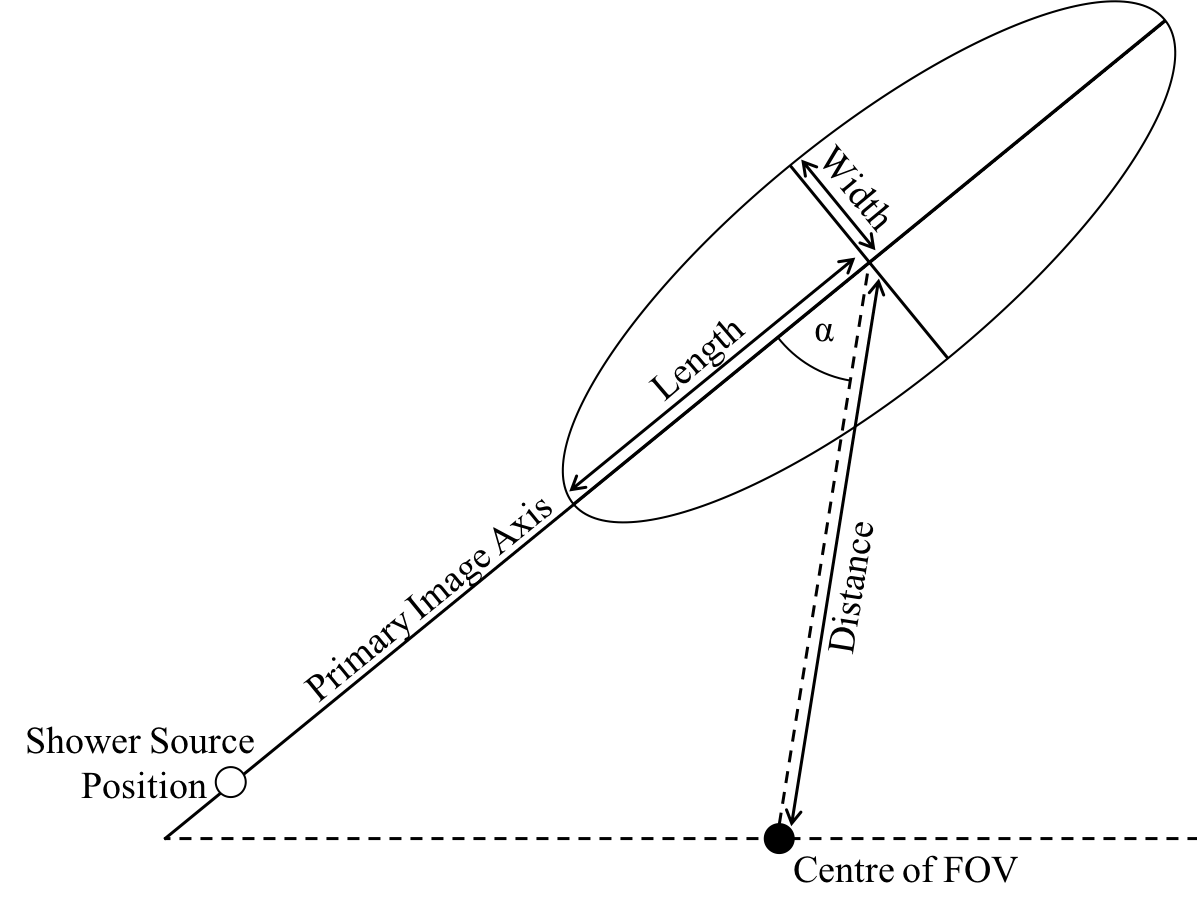
\includegraphics[width=\textwidth]{hillas} 
	\caption[Hillas Parametrisation Schematic.]{Schematic of the \textit{Hillas Parameters} used to describe the Cherenkov shower image ellipse.}
	\label{fig:hillas}
\end{figure}

Pixels containing signal from the Cherenkov shower are identified by an image cleaning method such as the tailcuts approach: any pixels above a certain signal threshold are kept, and any neighbouring pixels (to those that survive the first threshold) that are above a lower signal threshold are also kept. The thresholds are optimised per telescope using Monte Carlo simulations. The resulting pixels are then parametrised in terms of their second moments. This parametrisation is a predominant \gls{iact} analysis technique that has been utilised in the majority of \gls{iact} experiments. It was first formalised by \textcite{Hillas1985a} and has subsequently been known as the \textit{Hillas Parametrisation}. This technique exploits the elliptical shape of the gamma-induced shower images, and provides values for the centre of gravity of the ellipse, its primary axis position and orientation, its width, and its length (Figures~\ref{fig:hillas}). The \pkg{ctapipe} implementation of the \textit{Hillas Parametrisation} is defined by \textcite{Reynolds1993}.

\subsection{Direction Reconstruction}

\begin{figure}
\begin{minipage}[t]{.49\textwidth}
  \centering
  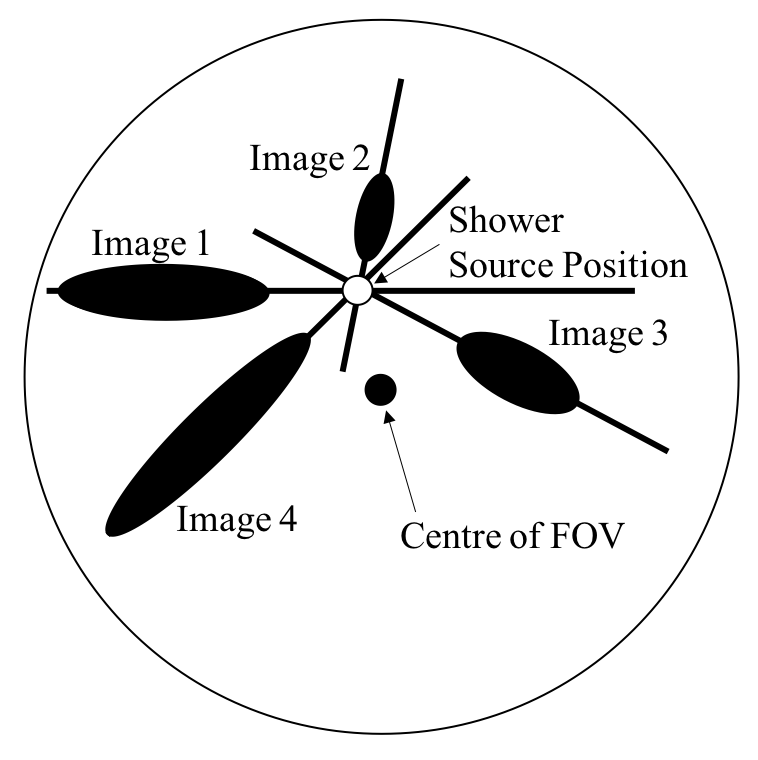
\includegraphics[width=0.92\textwidth]{source_location} 
  \captionof{figure}[Shower source location reconstruction.]{Reconstruction of the source location on the sky for the shower, achieved by superimposing the different views of the showers from different telescopes.}
  \label{fig:source_location}
\end{minipage}%
\hfill
\begin{minipage}[t]{.49\textwidth}
  \centering
  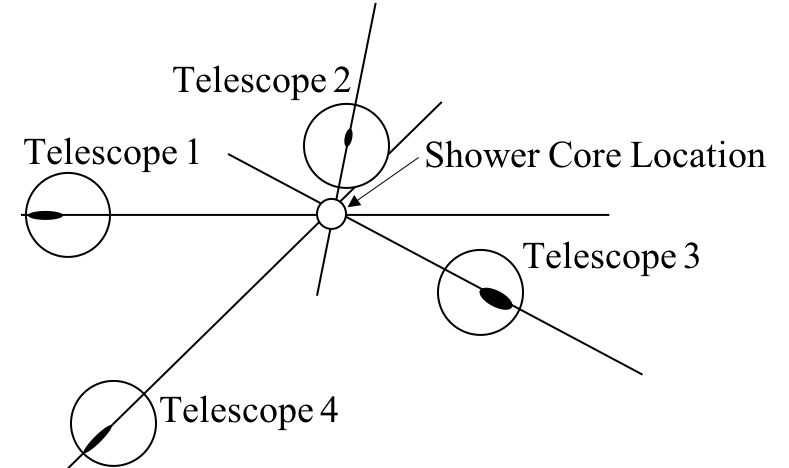
\includegraphics[width=\textwidth]{core_location}
  \captionof{figure}[Shower core location reconstruction.]{Reconstruction of the location of the shower core on the ground, achieved by combining the primary image axes at the relative telescope separations.}
  \label{fig:core_location}
\end{minipage}
\end{figure}

Through utilising the primary image axis that results from the \textit{Hillas Parametrisation}, the positional information about the shower can be obtained \cite{Daum1997,Cogan2006,Dickinson2010}. By superimposing the ellipses from different telescopes onto a single image (Figure~\ref{source_location}), the stereoscopic combination allows for the source position of the shower to be retrieved with simple geometry. As explained in Chapter~\otherch{refer to where it is explained that the two are the same, from introduction...}, this precisely \change{check wording in book} resolves the astrophysical-source position on the sky  for a gamma-ray shower. If, instead, the primary image axes are combined with the relative positional view of the telescopes (Figure~\ref{fig:core_location}), the core location of the shower in terms of ground coordinates may be obtained. For obtaining the intersections of the axes in both applications, the weighted-mean-direction of the intersections is typically calculated \cite{Eschbach2016,Bernlohr2013a}. While the extraction of the directional information is much more reliable through the use of the stereoscopic combination of the images, it is not impossible to estimate the direction of the source when only a single telescope is available. The primary challenge when performing this operation with a single telescope is the degeneracy in determining which direction along the primary image axis the source exists in. This is overcome with the \textit{disp} method developed by \textcite{Lessard2001}.

\subsection{Energy Reconstruction}

As aptly described by \textcite[][p.~16]{Dickinson2010}, ``determining of the energy of the progenitor of a particular air shower relies on a form of electromagnetic calorimetry''. Once the distance from the telescopes to the shower is known (from the core position), it can be coupled with the \textit{image size} (the total amount of integrated signal obtained from the Cherenkov shower) to obtain total energy released as Cherenkov light \cite{Cogan2006,Bernlohr2013a}. This is a proportional measure of the energy of the shower progenitor particle (Section~\otherch{section in introduction where it is shown that the majority of energy of the gamma-ray is released as Cherenkov light}).

\subsection{\textgamma-Hadron Discrimination}

\begin{figure}
	\centering
    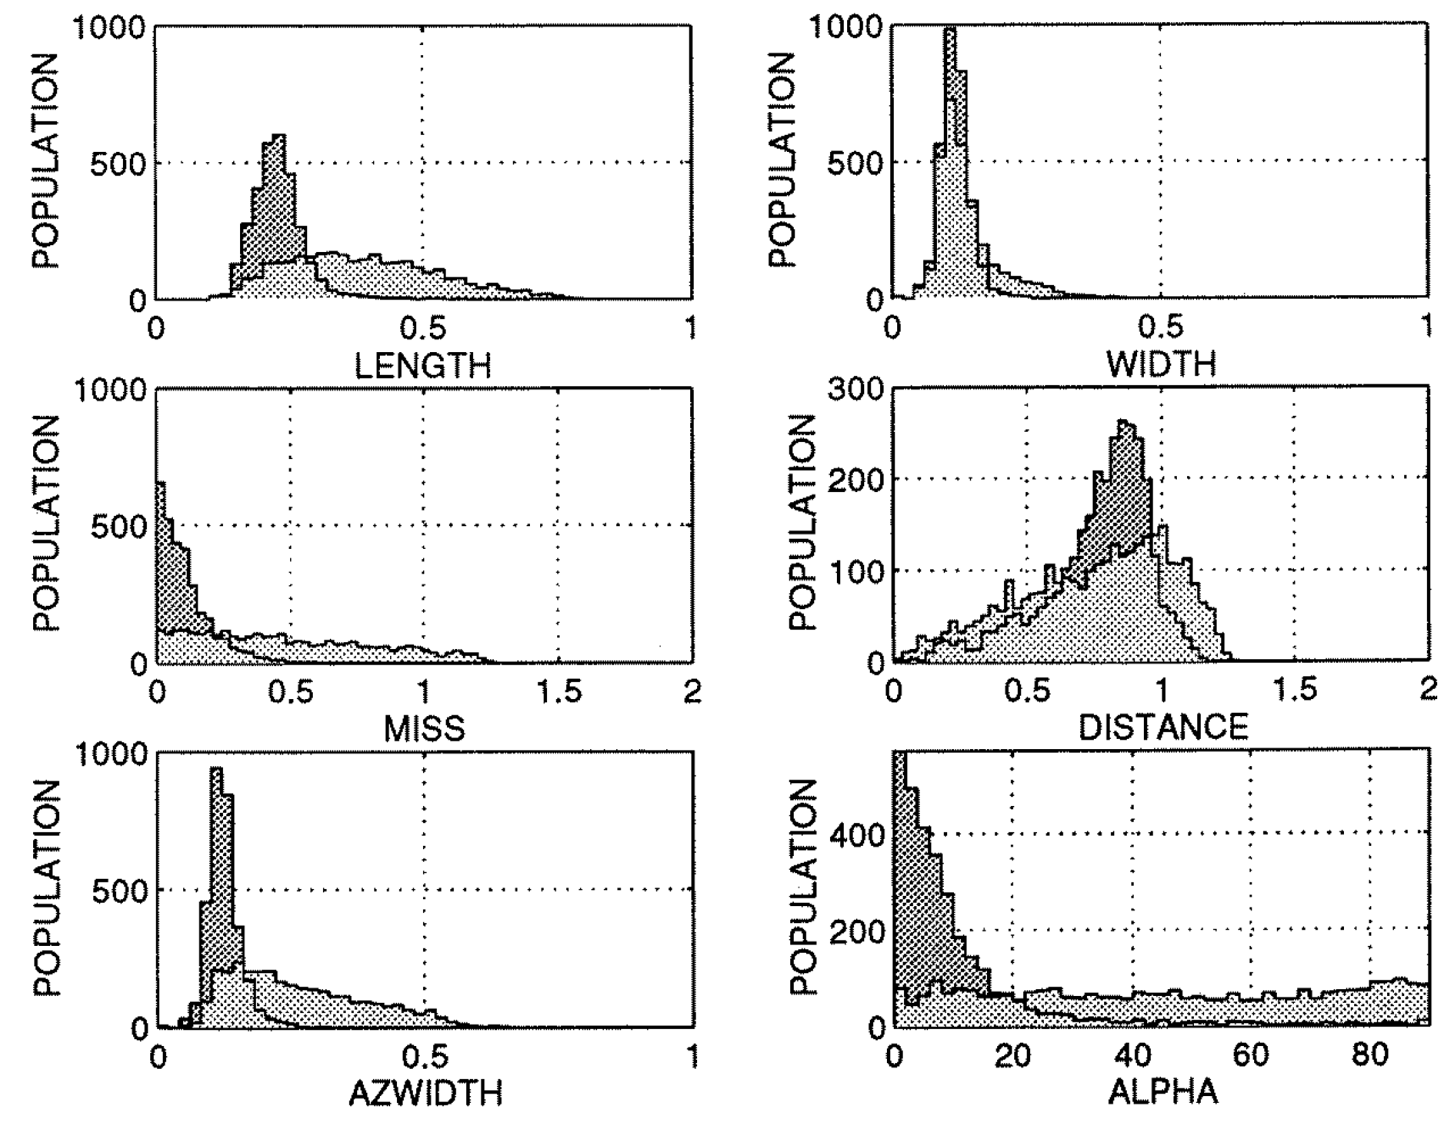
\includegraphics[width=\textwidth]{gamma_hadron_discrimination} 
	\caption[Discriminating between images of gamma-ray and hadron induced showers.]{Example of the differences in the distributions of \textit{Hillas Parameters} between simulated \textgamma-ray-induced showers (dark) and real hadronic-induced showers (light) for the Whipple \SI{10}{m} reflector \cite{Fegan1999a}.}
	\label{fig:gamma_hadron_discrimination}
\end{figure}

\begin{figure}
  \begin{subfigure}[b]{0.49\textwidth}
    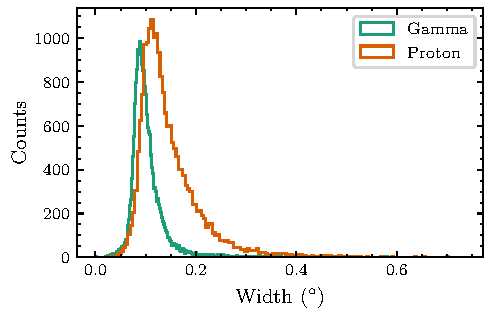
\includegraphics[width=\textwidth]{hillas_checs_width}
    \caption{}
    \label{fig:hillas_checs_width}
  \end{subfigure}
  \hfill
  \begin{subfigure}[b]{0.49\textwidth}
    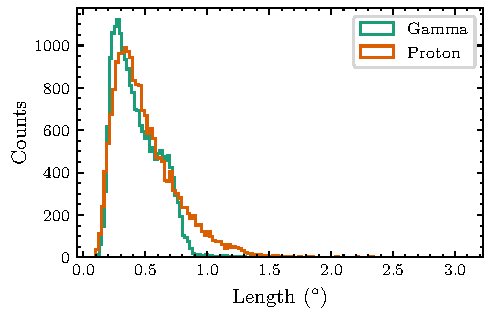
\includegraphics[width=\textwidth]{hillas_checs_length}
    \caption{}
    \label{fig:hillas_checs_length}
  \end{subfigure}
  \caption[Hillas width and length from CHEC-S simulations.]{The \textit{Hillas} width and length parameters extracted from Monte Carlo simulations of CHEC-S on the ASTRI telescope structure, for both gamma-ray and proton induced showers. The energy ranges simulated were \SIrange{2}{330}{TeV} for the gamma rays and \SIrange{6}{600}{TeV} for the protons. Each histogram contains approximately 20,000 shower images.}
    \label{fig:hillas_checs}
\end{figure}

The differences in image morphology between gamma-ray and hadronic showers is described in Chapter~\ref{ch1-intro}\otherch{describe differences in images in intro, and show perfect examples with MC of CHECS. Lessard gives precise information about the differences}. In traditional \gls{iact} analysis, these differences are quantified by the \textit{Hillas Parameters}. Gamma-ray showers typically exist within a narrow range of the parameters, while hadronic showers typically exhibit a broader spectrum of parameter values, as illustrated in Figure~\ref{fig:gamma_hadron_discrimination}. By creating an acceptance range for the \textit{Hillas Parameters}, the hadronic background can be excluded in a very simple way \cite{Dickinson2010,Fegan1999a,Hillas1996a}. However, at higher energies, the difference in morphology between gamma and hadron showers is limited, and it becomes harder to discriminate using simple cuts on the \textit{Hillas Parameters}. This is especially a problem for the \glspl{sst}, which are designed to operate within the gamma-ray energy range of \SIrange{1}{300}{TeV}. The distributions of the \textit{Hillas} width and length from simulations of \gls{chec-s} on the \gls{astri} telescope structure are shown in Figure~\ref{fig:hillas_checs}. More advanced techniques, such as the 
